\documentclass[12pt]{article}\usepackage[]{graphicx}\usepackage[]{color}
%% maxwidth is the original width if it is less than linewidth
%% otherwise use linewidth (to make sure the graphics do not exceed the margin)
\makeatletter
\def\maxwidth{ %
  \ifdim\Gin@nat@width>\linewidth
    \linewidth
  \else
    \Gin@nat@width
  \fi
}
\makeatother

\definecolor{fgcolor}{rgb}{0.345, 0.345, 0.345}
\newcommand{\hlnum}[1]{\textcolor[rgb]{0.686,0.059,0.569}{#1}}%
\newcommand{\hlstr}[1]{\textcolor[rgb]{0.192,0.494,0.8}{#1}}%
\newcommand{\hlcom}[1]{\textcolor[rgb]{0.678,0.584,0.686}{\textit{#1}}}%
\newcommand{\hlopt}[1]{\textcolor[rgb]{0,0,0}{#1}}%
\newcommand{\hlstd}[1]{\textcolor[rgb]{0.345,0.345,0.345}{#1}}%
\newcommand{\hlkwa}[1]{\textcolor[rgb]{0.161,0.373,0.58}{\textbf{#1}}}%
\newcommand{\hlkwb}[1]{\textcolor[rgb]{0.69,0.353,0.396}{#1}}%
\newcommand{\hlkwc}[1]{\textcolor[rgb]{0.333,0.667,0.333}{#1}}%
\newcommand{\hlkwd}[1]{\textcolor[rgb]{0.737,0.353,0.396}{\textbf{#1}}}%

\usepackage{framed}
\makeatletter
\newenvironment{kframe}{%
 \def\at@end@of@kframe{}%
 \ifinner\ifhmode%
  \def\at@end@of@kframe{\end{minipage}}%
  \begin{minipage}{\columnwidth}%
 \fi\fi%
 \def\FrameCommand##1{\hskip\@totalleftmargin \hskip-\fboxsep
 \colorbox{shadecolor}{##1}\hskip-\fboxsep
     % There is no \\@totalrightmargin, so:
     \hskip-\linewidth \hskip-\@totalleftmargin \hskip\columnwidth}%
 \MakeFramed {\advance\hsize-\width
   \@totalleftmargin\z@ \linewidth\hsize
   \@setminipage}}%
 {\par\unskip\endMakeFramed%
 \at@end@of@kframe}
\makeatother

\definecolor{shadecolor}{rgb}{.97, .97, .97}
\definecolor{messagecolor}{rgb}{0, 0, 0}
\definecolor{warningcolor}{rgb}{1, 0, 1}
\definecolor{errorcolor}{rgb}{1, 0, 0}
\newenvironment{knitrout}{}{} % an empty environment to be redefined in TeX

\usepackage{alltt}
\usepackage{amsmath,amssymb,mathrsfs,fancyhdr,syntonly,lastpage,hyperref,enumitem,graphicx,booktabs,tabularx}
\graphicspath{ {figure/} }
\hypersetup{colorlinks=true,urlcolor=black}

\topmargin      -1.5cm   % read Lamport p.163
\oddsidemargin  -0.04cm  % read Lamport p.163
\evensidemargin -0.04cm  % same as oddsidemargin but for left-hand pages
\textwidth      16.59cm
\textheight     23.94cm
\parskip         7.2pt   % sets spacing between paragraphs
\parindent         0pt   % sets leading space for paragraphs
\pagestyle{empty}        % Uncomment if don't want page numbers
\pagestyle{fancyplain}
\IfFileExists{upquote.sty}{\usepackage{upquote}}{}

\begin{document} \thispagestyle{empty}
\lhead{\today}
\chead{STAT544 Project}
\rhead{Ryan Goodrich}

\title{Feedstock availability for the biochemical conversion of corn stover to cellulosic ethanol}
\author{}
\date{}
\maketitle

\section{Introduction}
In 2005, Congress passed the Renewable Fuel Standard (RFS) and mandated the domestic consumption of ethanol, particularly grain ethanol.  Due in large part to various tax and other financial incentives, the ethanol industry boomed over the next few years and ethanol blended gasoline became more commonplace.  However, with rising food prices came the food vs fuel debate and concerns that biofuels were starving the poor \cite{Runge} and incentivizing the destruction of rainforests through indirect land use change \cite{Searchinger}.  Amidst these concerns, Congress directed the Environmental Protection Agency (EPA) to revise the RFS as part of the Energy Independence and Security Act of 2007 (EISA) with a shift away from grain ethanol.

While the RFS had made no specifications about the types of biofuels that were mandated, the RFS2 created categories for grain ethanol, advanced biofuels, cellulosic ethanol, and biodiesel, with each category having set requirements based on their green house gas (GHG) reductions compared to petroleum.  With concerns over land use impacts and the potentially substantial GHG reductions, cellulosic ethanol has received considerable attention and research funding over the past several years.

Although the end product is essentially the same as grain ethanol, cellulosic ethanol uses waste products such as municipal and agricultural waste and therefore has limited land use impact and does not directly compete with crops used for human consumption.  However, cellulosic ethanol has struggled to commercialize due to a number of complications in its production including feedstock collection and processing.  

The challenges in processing lie in the physical properties of the feedstocks.  Cellulosic ethanol is derived from lignocellulosic sources which have three main components: cellulose, hemicellulose, and lignin.  The cellulose and hemicellulose contain carbohydrate molecules that can be fermented in a similar fashion to the starches found in grains.  Lignin, however, cannot be easily fermented and must be separated from the other organic components for fermentation to take place.  Since lignin is covalently linked to the carbohydrates chains present in cellulose and hemicellulose, its removal from the lignocellulosic feedstock has proved challenging.  Only with recent advances in the production of cellulase enzymes designed to break the glycosidic bonds between carbohydrate molecules has cellulosic ethanol production become commercially viable.  This is evidence by the anticipated opening of two biochemical plants in Nevada and Emmetsburg, Iowa set to go commercial later this year.

Despite the production advances, feedstock collection and transportation still pose serious challenges to the commercial success of these plants.  In a typical plant, as the output grows a plant is able to take advantage of economies of scale which lower the per unit cost of the end product.  With the corn stover used for each of these upcoming plants however, the cost of transporting the feedstock to the plant grows as production capacity increases.  As shown in Wright and Brown (2007) \cite{Wright and Brown}, this implies that there is an optimal plant size for these biochemical plants due to the fact that plant costs and feedstock collection costs move in opposite directions as capacity increases.

Transportation costs have proven to be even more costly due to the limited willingness of farmers to provide their corn stover to biorefineries.  Corn stover, in some quantity, is typically left on the field following harvest to maintain soil carbon and provide nutrients for the following season.  Research has shown that at least some portion of the stover can be removed without damaging long-term soil quality but this quantity is highly dependent upon the particular acre and is not a widely agreed upon value.  Due to the uncertainty surrounding the sustainable quantity of removable stover, farmers have been hesitant to provide stover and feedstock collection costs for the DuPont and Poet plants opening later this year have proven to be higher than anticipated.  Because of these complications, there is a growing interest in the realities of the feedstock collection process.

In this analysis, I investigate the uncertainty surrounding the quantity of stover available to a cellulosic plant and in particular, I estimate the distance that the plant must travel to collect its feedstock input as a function of the plant's capacity.

\section{Methodology}

The focus here is on a plant which utilizes the production process now described.  Once the corn stover feedstock is present at the plant, it undergoes a dilute-acid pretreatment which breaks down the long chains of cellulose and converts much of the hemicellulose to sugar.  The feedstock then undergoes simultaneous enzymatic hydrolysis and fermentation.  The cellulase enzymes mentioned in the introduction are used in this step to convert the cellulose down into glucose which is then fermented along with the sugars present after the pretreatment step.  Finally, well-known distillation techniques are used to recover the anydrous ethanol.

To estimate the range of distances in which corn stover needs to be hauled into a plant of this kind, a simulation technique is used in which farmers with characteristics typical to Iowa are assumed to be uniformly distributed around the plant and the biorefinery selects the nearest willing farmers until the production quota is met.  To perform these simulations, I make use of relationships between feedstock and capacity as well as corn grain production and the corresponding corn stover production.

\subsection{The Feedstock-Capacity Relationship}

The quantity of feedstock necessary to produce a desired quantity of ethanol follows a transmission equation which converts stover to cellulosic ethanol according to the energy efficiency of the biomass to liquid process previously described.  This production efficiency is assumed to be 48\% following from a recent study by the National Renewable Energy Laboratory \cite{NREL}.  Since this percentage represents the proportion of the energy in the feedstock that remains in the end product, variables are converted into an energy basis.

Following from Wright et al. (2008), stover is assumed to take an energy content of 19.5 MJ/kg \cite{Wright et al} while gasoline is assumed to contain 120 MJ/gallon.  Taking the standard assumption that ethanol contains two-thirds the energy content of gasoline, the transmission equation can be parameterized as follows:

\begin{equation} \tag{1}
F = M \frac{E_{g}}{E_{etoh}} \frac{E_{etoh}}{E_{stover}*\eta_{BTL}}
\end{equation}

where F is the total quantity of corn stover in units of kilograms per year, $E_{etoh}$ is the energy content of ethanol, $E_{stover}$ is the energy content of corn stover, $E_g$ is the energy content of gasoline, $\eta_{BTF}$ is the fuel efficiency of the biomass-to-liquid process, and M is the plant capacity given in units of gge per year.

Using these parameters it is easy to calculate that for a plant the size of DuPont, which is expected to produce 20 million gallons of gasoline equivalen pper year, we would anticipate the need for around 171 million kilograms of corn stover.  Equivalently, DuPont's production process requires a little more than 188,000 tons per year.

\subsection{The Corn Grain-Corn Stover Relationship}

In order to approximate the stover available in the surrounding area of the plant, the first step is to estimate the production of corn stover on a given acre.  To do so I use a modified version of the technique developed by Grahem et al. (2007) \cite{Graham et al} in which corn stover production is a function of corn grain yield.  The conversion in this technique is accomplished through use of the dry weight harvest index, a measurement of the grain weight to the total weight of the plant.  Additionally, since corn grain production is reported in units of bushels an assumption on the dry grain mass of a bushel of corn must be made to convert to units of mass.  This parameterized as:

\begin{equation} \tag{2}
s_a = y_a * dgm * \frac{1-HI}{HI}
\end{equation}

where $s_a$ represents the kilograms of stover produced on acre a, $y_a$ represents the bushels of grain produced on acre a, dgm represents the dry grain mass in kilograms per bushel and HI represents the dry weight harvest index.  Note that since HI is the ratio of the weight of the grain to the total weight of the plant, 1-HI is the ratio of the weight of the stover to the total weight of the plant.

As mentioned previously, corn grain collection is heavily influenced by the willingness of farmers to participate in the collection process as well as the amount of stover, that can be sustainably removed from an acre.  To account for these two phenomenon, the above equation is modified into terms of the amount of stover that can be collected from a particular farmer:

\begin{equation}\tag{3}
s_f= r*p_f*dgm * \frac{1-HI}{HI}* \sum_{a=1}^{a_f} (y_a)  = b*p_f*dgm*\frac{1-HI}{HI}*y_f*a_f
\end{equation}

where $s_f$ is the amount of stover that con be collected from farmer f, b represents the proportion of stover that the biochemical plant proposes to remove, $p_f$ is an indicator function representing whether or not the farmer is willing to participate and $a_f$ is the number of acres harvested by farmer f.  $y_f$ is taken to be the average yield on the acres harvested by farmer f.  I.e., $y_f=\overline{y_a}_f$.

\subsection{Feedstock Uncertainty}

From the perspective of the biorefinery, the yield and area harvested of a participating farmer are random.  Likewise, since the decision of a given farmer to provide its stover or not is not well understood, farmer participation can appear random as well.  To capture this, the following distributional assumptions are made:

\begin{equation}\tag{4}
y_f \stackrel{iid}{\sim} pert(\alpha,\beta,l,u)
\end{equation}
\begin{equation}\tag{5}
a_f \stackrel{iid}{\sim} lognormal(\mu, \sigma^2)
\end{equation}
\begin{equation}\tag{6}
p_f \stackrel{iid}{\sim} bernoulli(\theta)
\end{equation}

Where each variable is assumed to be drawn from a distribution commmon to the state of Iowa.  Note that the modified pert distribution, although uncommon in many fields, is widely used in the scientific literature on corn yields and is an extension of the standard beta distribution to the support (l,u) through the linear transformation given by the equation:

\begin{equation}\tag{7}
y_f = l+(u-l)*x_f 
\end{equation}

where $x_f \sim beta(\alpha,\beta)$.

To facilitate the analysis, assumptions are made on the parameters.  The dry weight harvest index is taken to be 0.5, as reported by Gupta et al (1979) \cite{Gupta}.  The dry grain mass takes the value of 21.5 kg following from Wilcke and Wyatt (2002) \cite{Wilcke and Wyatt}.  The value of $\theta$ follows from a recent survey \cite{Tyndall} which finds that the proportion of farmers interested in harvesting feedstock for sale to a biorefinery to be 0.23 for north central Iowa, a likely location for the biorefinery.  Finally, the value for r, the portion of stover proposed to be removed, is set to 0.30.  This assumption matches the proportion that Graham finds could be removed sustainably given current rotation and tillage practices.

The parameters of the distribution for yield are determined through a method of moments estimation using county level data collected from the USDA's National Agricultural Statistics Service for the years 2004-2013.  This time frame is selected to minimize the influence of the time trend in yield growth which has leveled off in recent years.  After performing the inverse of the linear tranformation described above, it is found that $x_f \sim beta(5.6224,2.0514)$ fits the data well, as shown in the attached figure.

The area harvested for a farmer f follows from the most recent NASS survey data.  This data set is interval censored, placing farmers into one of six categories according to the number of acres they harvest.  Due to this data format, a Gibbs sampler is run in JAGS to fit this censored data to a lognormal distribution.

\begin{equation}\tag{8}
I(log(a_f) \in [log(L),log(U)) \sim normal(log(\mu),log(\sigma^2)[log(L),log(U)]
\end{equation}
\begin{equation}\tag{9}
\mu \sim normal(\tau,v^2)[0,\infty)
\end{equation}
\begin{equation}\tag{10}
\sigma^2 \sim invgamma(\alpha,\beta)
\end{equation}

where equation 8 applies to each of the six intervals.  Values for the prior parameters are chosen after an examination of the data and publicly available information.  Specifically, Excel's solver is used to minimize the sum of the squared differences between the percent of the data within a given interval and the percent of the assumed underlying lognormal distribution within that same interval subject to the constraint that the mean of the distribution equals 333 \cite{Iowa Quick Facts}.  The results of this operation suggest means for $\mu$ and $\sigma^2$ of 155.8869 and 3.428357, respectively.

Using these results, the parameters of the prior distribution are selected so that the mean of each distribution match the above results and the variance is sufficiently large.  This results in the following distributions:

\begin{equation}\tag{11}
\mu \sim normal(log(155.8869),log(20))[0,\infty)
\end{equation}
\begin{equation}\tag{12}
\sigma^2 \sim invgamma(2,log(3.428357))
\end{equation}

These prior distributions are placed into the Gibbs sampler, which is used to update $\alpha$ and $\beta$ using the censored data.  The results of this sampling, as shown in the attached figure, indicate that the prior distributions have converged and vary reasonably about their means.

\subsection{Distance Estimation}

To estimate the furthest distance that corn stover will need to be hauled to the centralized biorefinery, a circle around the biorefinery with an area equal to the state of Iowa is hypothesized in which farmers are uniformly distributed.  To account for the fact that roads do not run in a straight line, a tortuousity factor is used.  This factor represents the average distance travelled divided by the straight line distance between the two points.  While this factor has been shown to be as high as 3 for undeveloped agricultural regions, I follow the assumption of Wright and Brown \cite{Wright and Brown}, and take the value to be 1.5 for the area involved.  The distance that a given farmer is from the biorefinery is then assumed to be distributed as:

\begin{equation}\tag{13}
d_f \sim Unif(0,1.5*(\frac{56271.55}{\pi})^{0.5})
\end{equation}

\section{Simulation Results and Conclusions}

To match the farmer density of the state of Iowa, 50095 farmers are simulated to match the number of operations existing in the last NASS survey.  For each of these farmers, an area harvested, yield, distance, and willingness to participate are randomly drawn.  Using these draws, the amount of collectible stover per farm is calculated and used to form the cumulative quantity of stover as a function of distance.  Finally, distance is given as a function of capacity following from equation 1.  We can see from the plot that, unsurprisingly, capacity shows a linear relationship with distance.  This draws from the assumptions of homogeneity of farmers and their uniform density across the region.

What is of particular interest here is the sensitivity of this relationship to the parameters involved.  The experience at DuPont indicates that some of these parameters have been overestimated, with the likely candidates being the participation rate and the efficiency of the biomass to liquids process.  With regards to these variables, 6 scenarios are considered.  The participation rate is allowed to take the base level at 23\%, the statewide interest level of 17\% and a low value of 12.5\%.  These are selected following the Tyndall survey paper in which north central Iowa indicated the highest regional interest at 23\% and northeast Iowa indicated the lowest interest at around 12\%.  Since the biomass to liquids efficiency parameter depends on the energy efficiency of an enzymatic hydrolysis and co-fermentation process which has been untested at commercial scale, this parameter is allowed to vary by $\pm 10$\%.

It can be seen from the graphs that both factors heavily influence the slope of the relationship.  This has strong implications for the economic feasibility of the production process as it indicates that the feedstock costs are highly variable and have the potential to be extremely limiting to plant capacity.  To put things in perspective, the typical corn grain ethanol plant has a capacity of around 50 million gge per year.  The results here indicate that a corn stover ethanol plant operating at that capacity could be hauling in feedstock from between 20 and 40 miles away, based only on the variability in these two factors.

\begin{thebibliography}{25}

\bibitem{Graham et al} Graham, Robin Lambert, et al. "Current and potential US corn stover supplies." Agronomy Journal 99.1 (2007): 1-11.

\bibitem{Gupta} Gupta, S. C., C. A. Onstad, and W. E. Larson. "Predicting the effects of tillage and crop residue management on soil erosion." Journal of Soil and Water Conservation 34 (1979).

\bibitem{Iowa Quick Facts} Iowa Agricultural Statistics. 2013.  Available at www.iowaagriculture.gov/quickfacts.asp (accessed 23 April 2014).

\bibitem{Linden et al} Linden, Dennis R., C. Edward Clapp, and Robert H. Dowdy. "Long-term corn grain and stover yields as a function of tillage and residue removal in east central Minnesota." Soil and Tillage Research 56.3 (2000): 167-174.

\bibitem{Montross et al} Montross, M.D., R. Prewitt, S.A. Shearer, T.S. Stombaugh, S.G. McNeil, and S. Sokhansanj.  2002.  Economics of collection and transportation of corn stover.  ASAE Paper 036081 presented at the Annual International Meeting of the American Society of Agricultural Engineers, Las Vegas, NV. 27-31 July 2003.  ASAE, St. Joseph, MI.

\bibitem{NREL} Humbird, D., et al. Process Design and Economics for Biochemical Conversion of Lignocellulosic Biomass to Ethanol National Renewable Energy Laboratory Report NREL. TP-5100-47764, 2011.

\bibitem{Runge} Runge, C. Ford, and Benjamin Senauer. "How biofuels could starve the poor." Foreign affairs (2007): 41-53.

\bibitem{Searchinger} Searchinger, Timothy, et al. "Use of US croplands for biofuels increases greenhouse gases through emissions from land-use change." Science 319.5867 (2008): 1238-1240.

\bibitem{Tyndall} Tyndall, John C., Emily J. Berg, and Joe P. Colletti. "Corn stover as a biofuel feedstock in Iowa’s bio-economy: an Iowa farmer survey." Biomass and bioenergy 35.4 (2011): 1485-1495.

\bibitem{USDA-NASS} USDA-NASS. 2007.  Agricultural statistics data base (quick stats).  Available at www.nass.usda.gov (accessed 23 April 2014).  USDA-NASS, Washington, D.C.

\bibitem{Wilcke and Wyatt} Wilcke, William, and Gary Wyatt. "Grain Storage Tips." Twin Cities, MN, The University of Minnesota Extension Service, the University of Minnesota (2002).

\bibitem{Wright and Brown} Wright, Mark, and Robert C. Brown. "Establishing the optimal sizes of different kinds of biorefineries." Biofuels, Bioproducts and Biorefining 1.3 (2007): 191-200.

\bibitem{Wright et al}  Wright, Mark M., Robert C. Brown, and Akwasi A. Boateng. "Distributed processing of biomass to bio‐oil for subsequent production of Fischer‐Tropsch liquids." Biofuels, bioproducts and biorefining 2.3 (2008): 229-238.

\end{thebibliography}

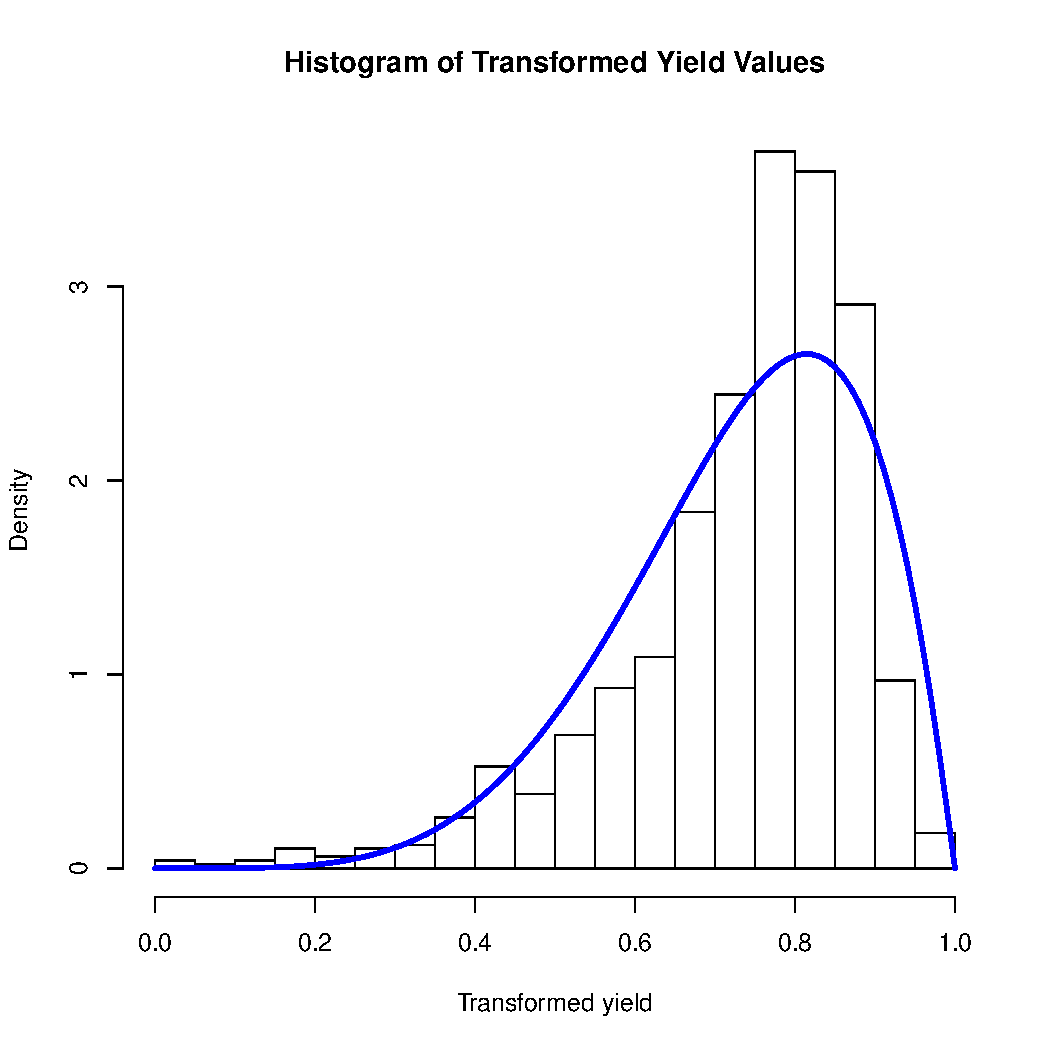
\includegraphics{Histogram_of_yield_fit}
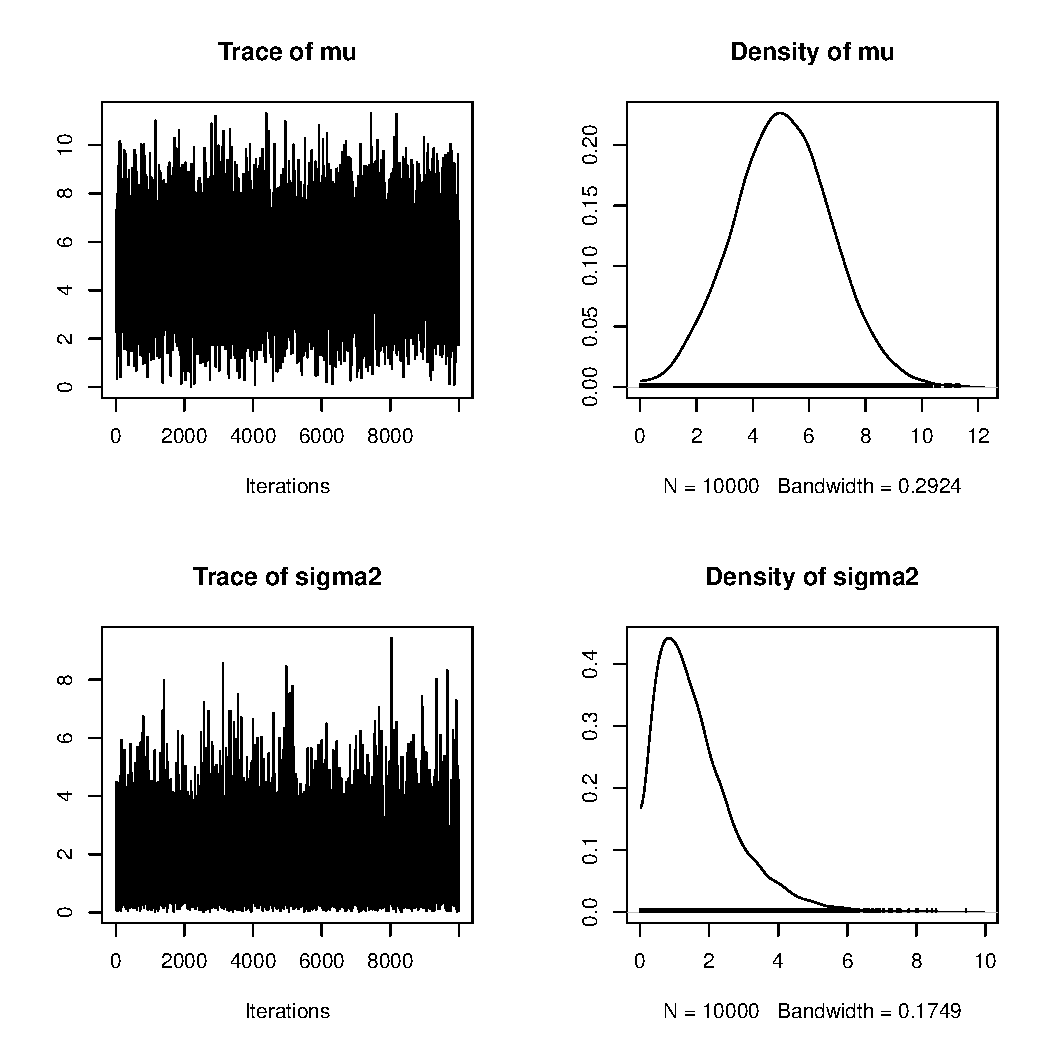
\includegraphics{Sampler}
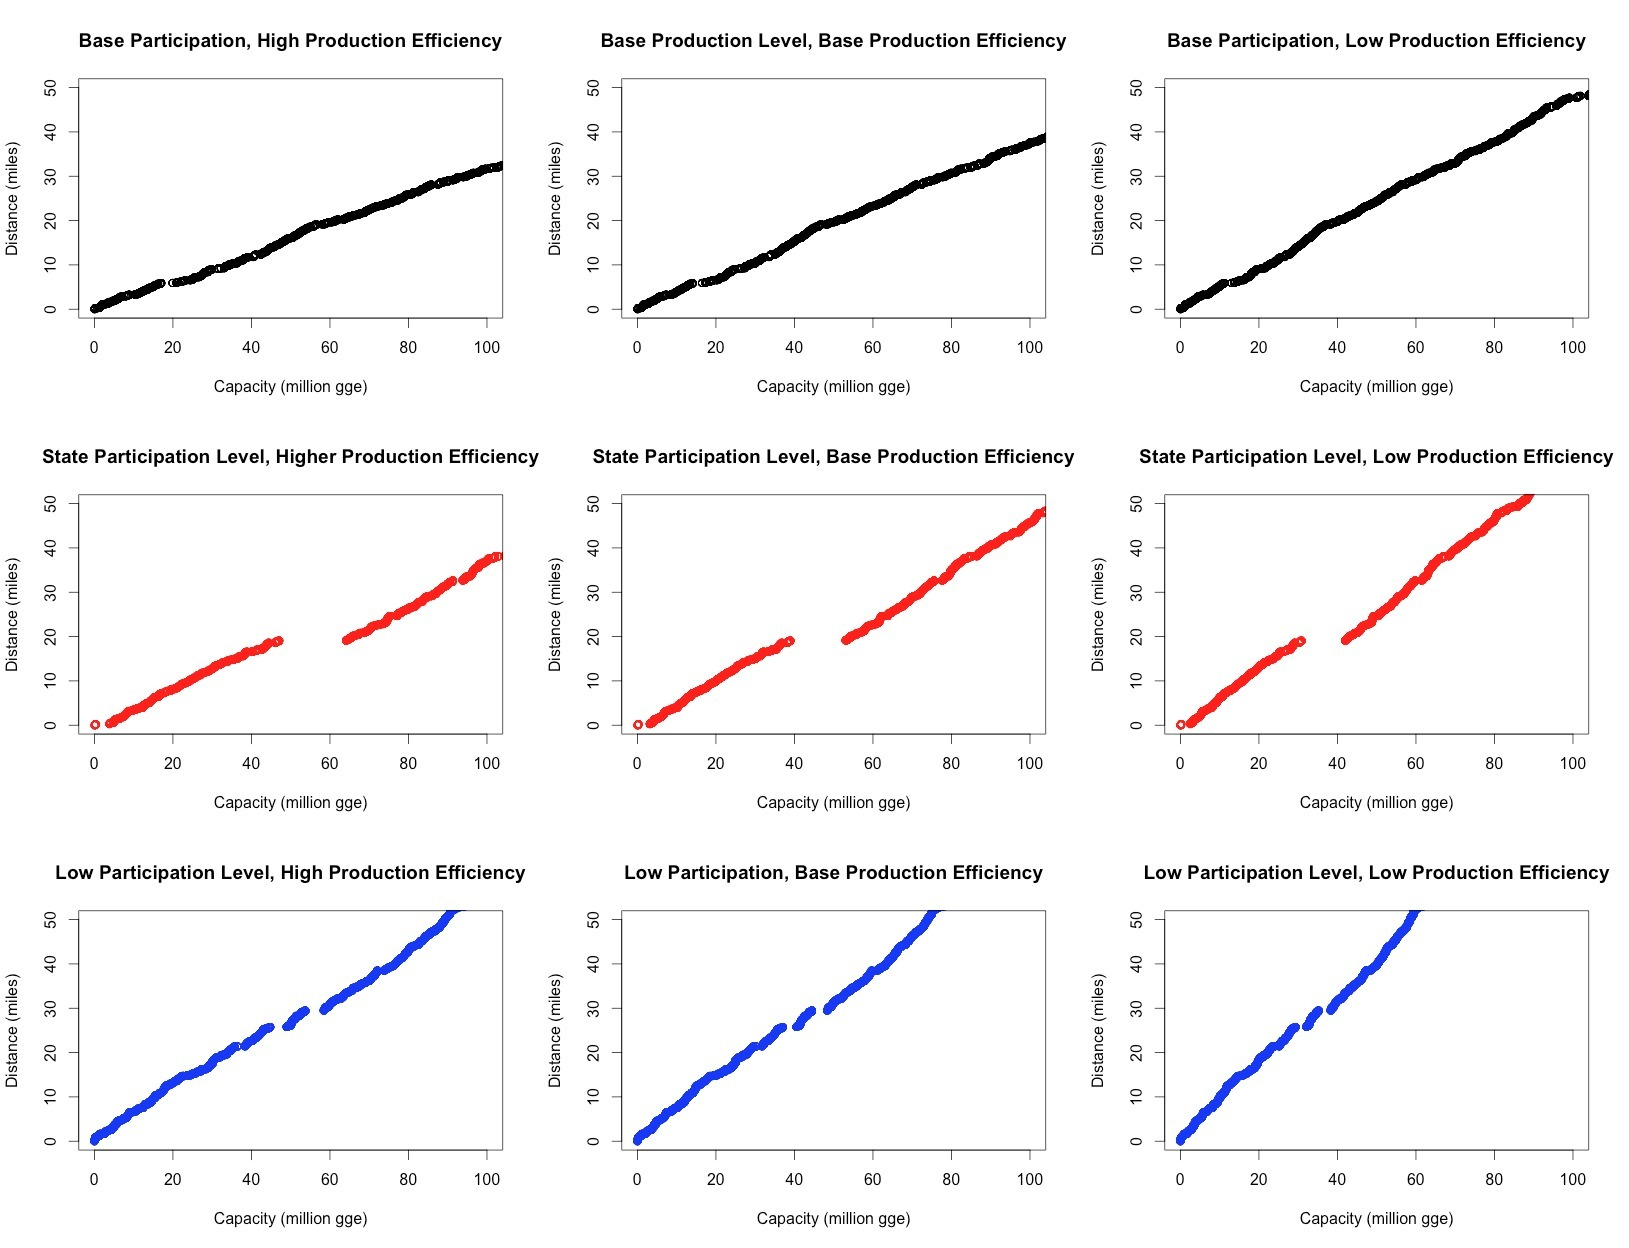
\includegraphics{part_prod}

\end{document}
